%Ne pas numéroter cette partie
\part*{Annexes}
%Rajouter la ligne "Annexes" dans le sommaire
\addcontentsline{toc}{part}{Annexes}

\addtocontents{toc}{\protect\setcounter{tocdepth}{0}}

\appendix
\section{Tableaux des différences finies}
Pour la méthode  différences finies, on a utilisé les tableaux suivants pour les schémas des différents ordres, tirés de "Méthodes Numériques, Équations aux Dérivées Partielles (EDP)" de l'institut d'optique Paritech.

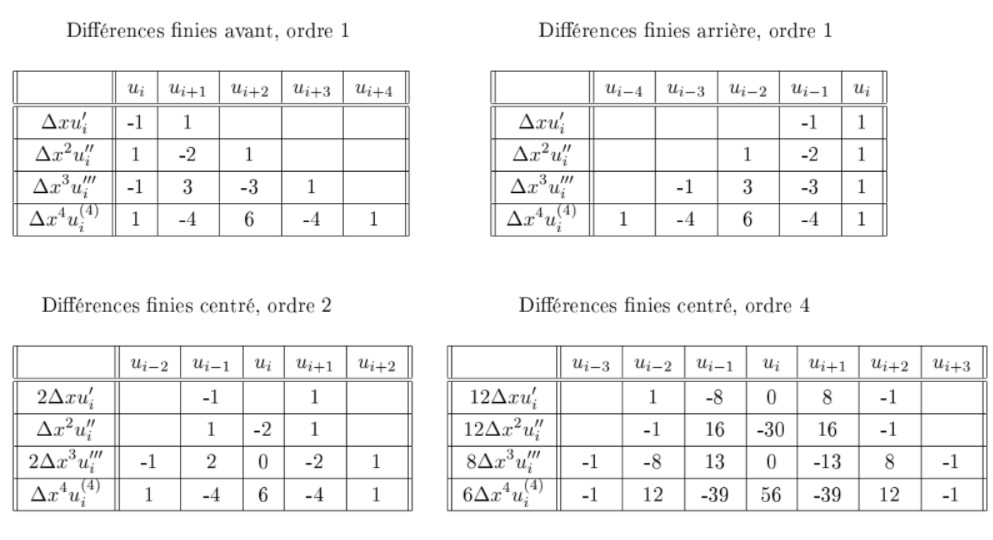
\includegraphics[width=1\textwidth]{./annex1}~\\[1cm]

\section{Solutions pour la partie comparaison}
\begin{figure}[H]
\begin{minipage}[b]{.46\linewidth}
\centering\epsfig{figure=exact.png,width=\linewidth}
\caption{Solution exacte
    \label{fig1}
    }
\end{minipage} \hfill
\begin{minipage}[b]{.46\linewidth}
\centering\epsfig{figure=explicite.png,width=\linewidth}
\caption{Euler explicite\label{fig2}}
\end{minipage}
\end{figure}

\begin{figure}[H]
\begin{minipage}[b]{.46\linewidth}
\centering\epsfig{figure=implicite.png,width=\linewidth}
\caption{Euler implicite\label{fig1}}
\end{minipage} \hfill
\begin{minipage}[b]{.46\linewidth}
\centering\epsfig{figure=RK.png,width=\linewidth}
\caption{Runge-Kutta \label{fig2}}
\end{minipage}
\end{figure}

\section{Algorithmes}
\subsection{Euler explicite}

\begin{enumerate}
    \item Initialisation des pas $\Delta x$ et $\Delta t$\\
    Initialisation des nombre de points du temps Nt et du nombre de points de l'espace Nx
    
    \item Calculs des conditions initiales $u^0_i$ et de $u^1_i$
    
    \item Calcul de la matrice trigonale A
    
    \item Tant que n<Nt faire:
        \begin{itemize}
        \item Calculs de $U^{n+1}_i$ : $U^{n+1}_i = A.U^{n}_i - U^{n-1}_i + C_i$\\
        \end{itemize}
    
\end{enumerate}

\subsection{Euler implicite}
\begin{enumerate}
    \item Initialisation des pas $\Delta x$ et $\Delta t$\\
    Initialisation des nombre de points du temps Nt et du nombre de points de l'espace Nx
    
    \item Calculs des conditions initiales $u^0_i$ et de $u^1_i$
    
    \item Calcul de la matrice trigonale A et de son inverse $A^{-1}$
    
    \item Tant que n<Nt faire:\\
        \begin{itemize}
            \item Calcul de $U^{n+1}_i$: $U^{n+1}_i = A^{-1}(U^{n}_i - \frac{1}{2}.U^{n-1}_i)$
        \end{itemize}
    
\end{enumerate}

\subsection{Runge-Kutta}
Algorithme utilisé dans le code python:
\begin{enumerate}
    \item Initialisation des pas $\Delta x$ et $\Delta t$\\
    Initialisation des nombre de points du temps Nt et du nombre de points de l'espace Nx
    
    \item Calculs des conditions initiales $u^0_{i}$ et de $(\frac{\partial u^n_{i}}{\partial t})^0_{i}$
    
    \item Tant que n<Nt faire:\\
     Tant que i<Nx faire:
        \begin{itemize}
            \item Calcul de $((k_0)_{i})$
            \item Calcul de $((l_0)_{i})$
            \item Calcul de $((k_1){i})$
            \item Calcul de $((l_1)_{i})$
            \item ...
            \item Calculs de $u^{n+1}_{i}$ et $(\frac{\partial u^n_{i}}{\partial t})^n_{i}$
        \end{itemize}
    
\end{enumerate}

\section{Lien Github}
Lien vers le répertoire Github contenant les différents codes python utilisés au cours du projet:\\
\url{https://github.com/Rudiio/Projet-Musique.git}

\section{Tests complémentaires pour la méthode de Runge-Kutta}
\begin{figure}[H]
\begin{minipage}[b]{.46\linewidth}
\centering\epsfig{figure=55.png,width=7cm}
\caption{
        $\Delta x= 5^{-2}m $\\
        $\Delta t= 10^{-7}s$\\
        $\lambda = 6.8.10^{-4}$
    \label{fig1}
    }
\end{minipage} \hfill
\begin{minipage}[b]{.46\linewidth}
\centering\epsfig{figure=44.png,width=7cm}
\caption{$\Delta x= 5^{-3}m $\\ 
        $\Delta t= 10^{-6}s$\\
        $\lambda = 0.068$
        \label{fig2}}
\end{minipage}
\end{figure}

\begin{figure}[H]
\begin{minipage}[b]{.46\linewidth}
\centering\epsfig{figure=9_stab.png,width=7cm}
\caption{$\Delta x= 5^{-4}m $\\ 
        $\Delta t= 1.47.10^{-6}s$\\
        $\lambda = 1$
        \label{fig1}
        }
\end{minipage} \hfill
\begin{minipage}[b]{.46\linewidth}
\centering\epsfig{figure=10.png,width=\linewidth}
\caption{$\Delta x= 3^{-3} m $\\ 
        $\Delta t= 10^{-6}s  $\\
        $\lambda = 0.113$
        \label{fig2}}
\end{minipage}
\end{figure}
